% CS 6501 3D Computer Vision -- Project Mid-term Report (CVPR style)
\documentclass[10pt,twocolumn,letterpaper]{article}
\usepackage[pagenumbers]{cvpr}
\usepackage{cuted}
\usepackage{caption}
\usepackage{graphicx}
\graphicspath{{figures/}}
\usepackage{booktabs}
\usepackage{amsmath,amssymb}
\usepackage{microtype}
\definecolor{cvprblue}{rgb}{0.21,0.49,0.74}
\usepackage[pagebackref,breaklinks,colorlinks,allcolors=cvprblue]{hyperref}
\def\confName{CVPR}
\def\confYear{2027}
\usepackage{xspace}
\newcommand{\dB}{\,dB\xspace}
\newcommand{\step}[1]{\textbf{(#1)}}

\title{Open Free-Viewpoint Reconstruction of Athletes with Dynamic 3D Gaussians}
\author{Faizan Khan\\ University of Virginia\\ {\tt\small xdy6sg@virginia.edu}}

\begin{document}
\twocolumn[{%
\renewcommand\twocolumn[1][]{#1}%
\maketitle
\vspace{-2.2em}
\begin{center}
  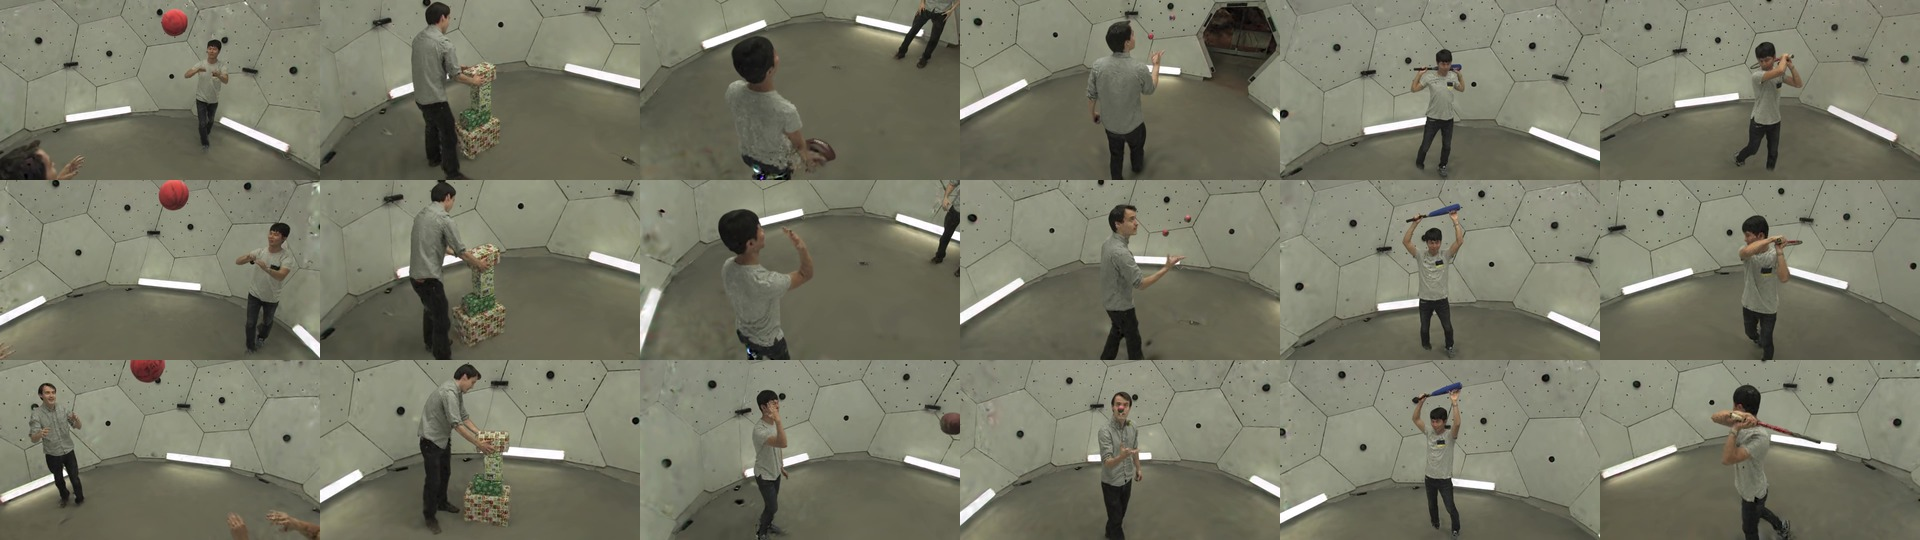
\includegraphics[width=\textwidth]{teaser.jpg}
  \vspace{-1.6em}
  \captionof{figure}{\textbf{Cinematic 3D replays made by our open pipeline.} Columns: basketball, boxes, football, juggle, softball, tennis. Rows: three moments of one automatically planned shot (push-in, freeze-time sweep, crane). No real camera stood at any of these viewpoints.}
  \label{fig:teaser}
\end{center}
\vspace{0.4em}
}]

\begin{abstract}
Some sports broadcasts now show replays where time stops and the camera flies around the athlete. The systems behind them, such as Arcturus and World Labs' Atlas, are closed, so it is hard to see how they work or how good they are. We build an open version. The input is synchronized video from many calibrated cameras. The output is a cinematic 3D replay with a free viewpoint, slow motion and freeze-time. The pipeline has four parts: preparing the data, building a 4D model with Dynamic 3D Gaussians (D3G), measuring it on cameras it never saw, and an automatic ``director'' that finds the key moment and plans a smooth camera path. On PanopticSports (six clips, 31 cameras), the 4D models score 27.0--29.3\dB PSNR and 0.89--0.91 SSIM on held-out cameras across all six sports. The director runs on all six sports with no per-clip tuning, and its camera motion is about 35$\times$ smoother than a path that blends the real camera poses.
\end{abstract}

%%%%%%%%%%%%%%%%%%%%%%%%%%%%%%%%%%%%%%%%%%%%%%%%%%%%%%%%%%%%%%%%%%%%%%
\section{Introduction}
\label{sec:intro}

A replay that can freeze time and move the camera anywhere shows things the real cameras missed: the release of a throw, the angle of a bat, a foot on a line. In class we saw World Labs' Atlas~\cite{worldlabs2026atlas}, which turns ``a handful of ordinary cameras into a bullet time multiview capture studio.'' Arcturus~\cite{arcturus} sells this idea to broadcasters: synchronized sensors around a venue, a radiance field for every moment stored as splats, and new views rendered from any position. Online, an engineer at Roboflow rebuilds players as textured 3D bodies from a single broadcast camera~\cite{mirrash2026b,mirrash2026}, building on Roboflow's open tools for detecting, tracking and identifying players~\cite{skalski2025roboflow}. Another posted a Gaussian splat of a World Series home run~\cite{middlecamp2026}. \cref{fig:insp} shows these sources.

None of them releases a full pipeline from video to replay, and none reports accuracy. We first tried the single-camera route ourselves. The novel views looked plausible, but we could not check them, because no other camera saw the scene. So we moved to synchronized multi-view video, where cameras held out from training give real images to compare against.

\noindent\textbf{Goal.} Given synchronized multi-angle video of an athlete, produce an immersive, cinematic 3D replay, and measure how faithful it is. Uses include broadcasting, coaching and AR/VR.

\noindent\textbf{Contributions.} (1) An open, end-to-end pipeline from synchronized video to a replay video, built on D3G~\cite{luiten2024dynamic} and run on a shared university GPU cluster (\cref{fig:workflow}). (2) An automatic director: it finds the key moment, picks a side-on view, flies a broadcast-style shot list, keeps clear of the players, and renders slow motion by blending the Gaussians between frames. It works on six different sports. (3) An evaluation of every step on all six sports: held-out image quality, stability over time, 3D motion tracks and replay smoothness.

\begin{figure}[t]
\centering
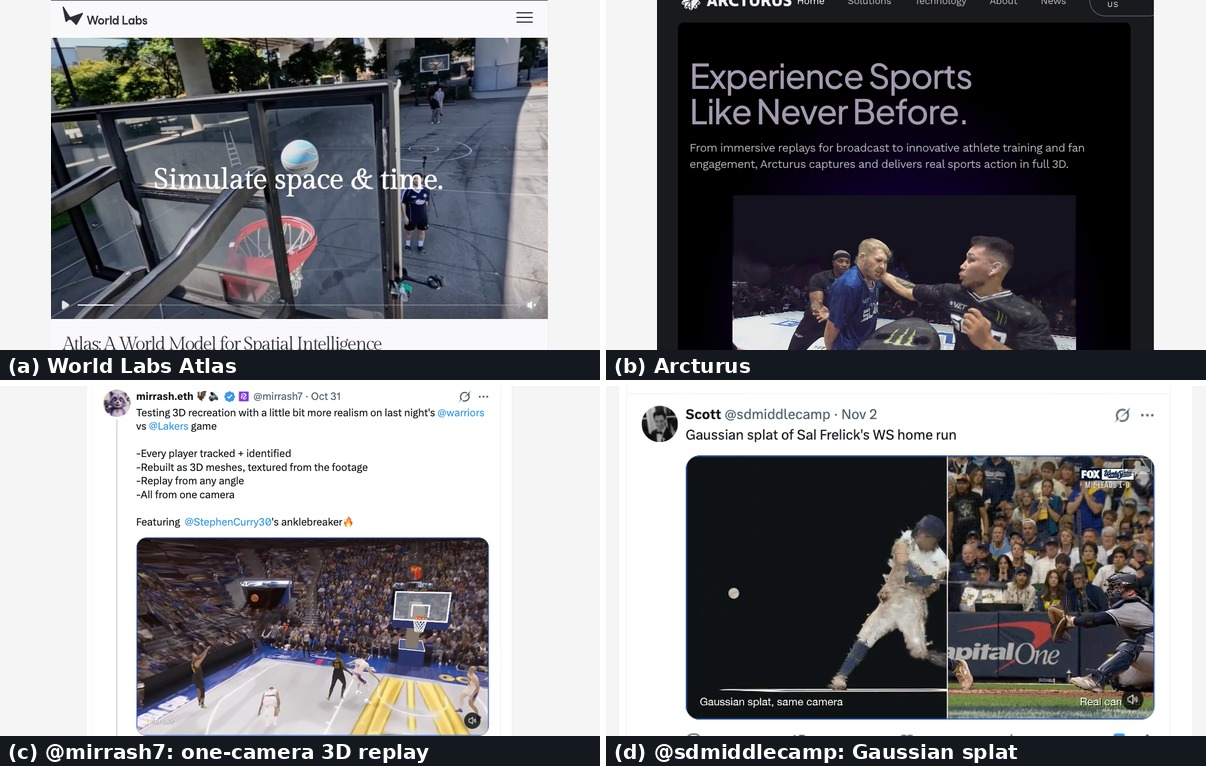
\includegraphics[width=\columnwidth]{inspiration.jpg}
\vspace{-1.6em}
\caption{\textbf{What inspired this project.} (a) World Labs' Atlas, shown in class~\cite{worldlabs2026atlas}. (b) Arcturus, volumetric sports replays for broadcast~\cite{arcturus}. (c) A 3D replay rebuilt from one broadcast camera by a Roboflow engineer~\cite{mirrash2026b}. (d) A Gaussian splat of a World Series home run next to the real camera~\cite{middlecamp2026}. Screenshots, Nov.\ 2026.}
\label{fig:insp}
\vspace{-1em}
\end{figure}

%%%%%%%%%%%%%%%%%%%%%%%%%%%%%%%%%%%%%%%%%%%%%%%%%%%%%%%%%%%%%%%%%%%%%%
\section{Background and Related Work}
\label{sec:related}

\noindent\textbf{Radiance fields and splatting.} NeRF~\cite{mildenhall2020nerf} stores a scene in a neural network and renders it by volume rendering. 3D Gaussian Splatting (3DGS)~\cite{kerbl3dgs} stores it as millions of small 3D Gaussians and renders them in real time by rasterization, which suits video. Both need calibrated cameras; in a real venue these come from structure-from-motion such as COLMAP~\cite{schoenberger2016sfm}.

\noindent\textbf{Dynamic scenes.} D3G~\cite{luiten2024dynamic} keeps one set of Gaussians for the whole clip and moves them frame by frame, with physical priors that keep neighbours moving together. Its Gaussians are persistent, so it also tracks every point in 3D. 4DGS~\cite{wu20244dgs} and Spacetime Gaussians~\cite{li2024spacetime} model motion with a deformation field or per-Gaussian curves. Feed-forward models from class, D4RT~\cite{zhang2025d4rt} and CoTracker3~\cite{karaev2024cotracker3}, recover depth and motion from video in one pass, but they do not aim at photoreal rendering from new viewpoints.

\noindent\textbf{Feed-forward reconstruction.} VGGT~\cite{wang2025vggt} and MapAnything~\cite{keetha2025mapanything} predict cameras and dense geometry from a set of images in one pass. RayZer~\cite{jiang2025rayzer} learns view synthesis without 3D labels, and WildRayZer~\cite{chen2026wildrayzer} extends it to scenes with moving content. pixelSplat~\cite{charatan2024pixelsplat}, MVSplat~\cite{chen2024mvsplat} and FSGS~\cite{zhu2024fsgs} build splats from few images of static scenes. Such models could one day replace our per-clip optimization with a single fast pass.

\noindent\textbf{Sports.} The CMU Panoptic Studio~\cite{joo2015panoptic} provides the multi-view data we use. Sports vision mostly targets tracking and pose~\cite{somers2024soccernet,jiang2024worldpose,skalski2025roboflow}, not photoreal views.

%%%%%%%%%%%%%%%%%%%%%%%%%%%%%%%%%%%%%%%%%%%%%%%%%%%%%%%%%%%%%%%%%%%%%%
\section{Dataset: PanopticSports}
\label{sec:data}

PanopticSports was released with D3G~\cite{luiten2024dynamic}. It is cut from the CMU Panoptic Studio~\cite{joo2015panoptic}, a geodesic dome lined with cameras, and comes from capture \texttt{161029\_sports1}. It has six clips of one or two people: \emph{basketball} (two players passing a ball), \emph{boxes} (stacking boxes), \emph{football} (throwing an American football), \emph{juggle} (juggling small balls), \emph{softball} (swinging a bat) and \emph{tennis} (swinging a racket). Each clip has 150 frames from 31 synchronized HD cameras, resized to 640$\times$360. The split is fixed: 27 cameras for training and 4 held out for testing. Every image comes with its camera calibration and a foreground mask, and each clip has a starting point cloud. The raw capture also has 3D body skeletons; we aligned them to the clips (clean frame $t$ $\approx$ raw frame $4059$--$4061{+}t$), and 83.2\% of the projected joints land on the foreground mask, which confirms the calibration.

%%%%%%%%%%%%%%%%%%%%%%%%%%%%%%%%%%%%%%%%%%%%%%%%%%%%%%%%%%%%%%%%%%%%%%
\section{Method}
\label{sec:method}

\begin{figure*}[t]
\centering
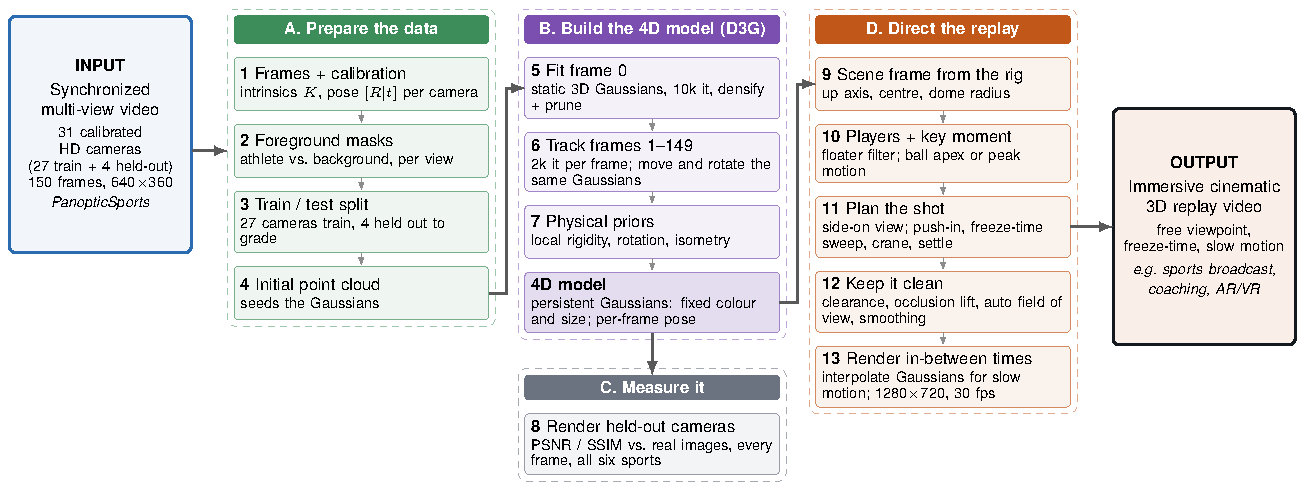
\includegraphics[width=\textwidth]{workflow.pdf}
\vspace{-1.6em}
\caption{\textbf{Workflow.} Synchronized multi-view video goes through four stages. A: prepare frames, calibration, masks, a train/test split and a starting point cloud. B: build the 4D model with Dynamic 3D Gaussians. C: measure it on held-out cameras. D: the director plans and renders the replay. Numbers match the steps in \cref{sec:method} and \cref{fig:stages}.}
\label{fig:workflow}
\vspace{-0.6em}
\end{figure*}

\begin{figure*}[t]
\centering
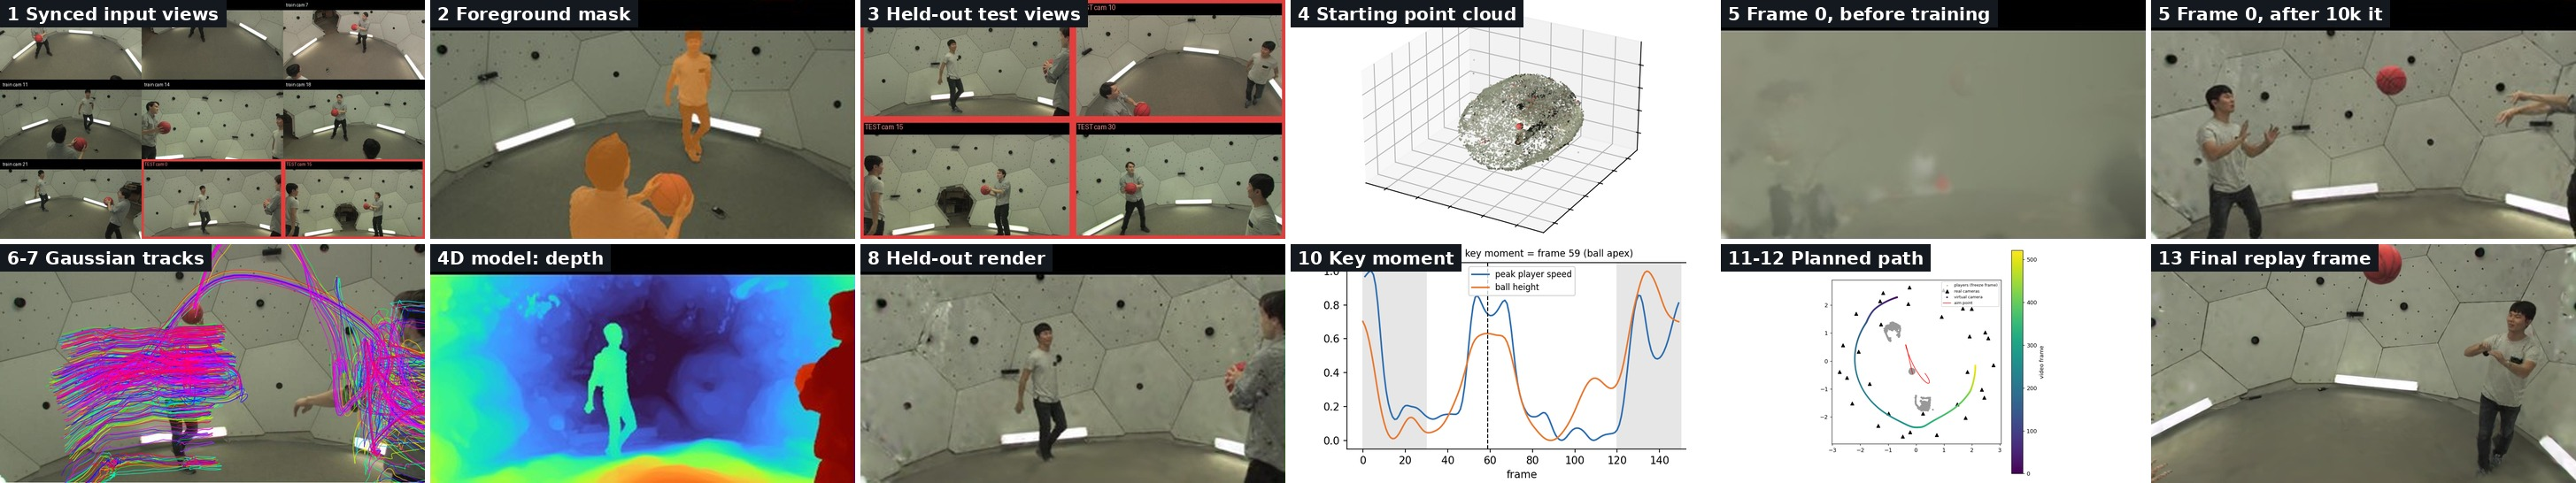
\includegraphics[width=\textwidth]{stages.jpg}
\vspace{-1.6em}
\caption{\textbf{Intermediate output after each step} (basketball). Numbers refer to the steps in \cref{fig:workflow}. Step 3 shows the 4 held-out test views (red). Step 10 plots normalized ball height and peak player speed; the dashed line is the chosen freeze frame.}
\label{fig:stages}
\vspace{-1em}
\end{figure*}

\cref{fig:workflow} shows the whole workflow and \cref{fig:stages} shows what comes out of each step. For every step we say what it does, why we need it, and what we got.

\noindent\textbf{Why this design should work.} We picked D3G over other dynamic models because its Gaussians persist through time. That gives us, for free, a 3D track for every point, which the director uses to find motion, and a clean way to render \emph{between} frames for slow motion. Arcturus describes the same recipe~\cite{arcturus}, so a careful open version should reach broadcast-like results in a controlled dome. Where we expect to beat the obvious baseline is the camera move: blending real camera poses inherits the rig's uneven spacing, while planning in the scene's own frame gives a smooth path wherever the cameras happen to be.

\noindent\textbf{A. Prepare the data.}
\step{1} \emph{Frames and calibration.} We load each camera's intrinsics $K$ and pose, which rendering needs exactly; we get 31 synced views per frame.
\step{2} \emph{Foreground masks} separate the athlete from the dome. D3G trains a foreground/background colour on each Gaussian against these masks, and later the director uses that label to find the players.
\step{3} \emph{Train/test split.} 27 cameras train the model; the other 4 are never used for training and only grade the result, so we can check views the model has not seen.
\step{4} \emph{Starting point cloud.} 3DGS needs points to start from. Each Gaussian starts at one of the 194k points of the released cloud, with its colour and an athlete/background label.

\noindent\textbf{B. Build the 4D model.}
\step{5} \emph{Frame 0} is fit like static 3DGS for 10k iterations with an $\ell_1$+SSIM image loss and a mask loss. Gaussians are split, cloned and pruned as needed. Before training the held-out render is a grey blur; after 500 iterations it is already at 27.9\dB, and the Gaussians grow from 194k to about 365k by the end.
\step{6} \emph{Frames 1--149.} Each frame starts from the previous one and gets 2k iterations. Colour, size and opacity stay fixed; only each Gaussian's position and rotation change, and background Gaussians stay put.
\step{7} \emph{Physical priors} keep this motion sensible: neighbouring Gaussians should move rigidly, rotate together and keep their distances~\cite{luiten2024dynamic}. The result is a 4D model whose Gaussians trace the athlete's motion over 150 frames.

\noindent\textbf{C. Measure it.}
\step{8} We render the 4 held-out cameras at every frame and compare with the real images (PSNR, SSIM). We do this for all six sports.

\noindent\textbf{D. Direct the replay.}
\step{9} \emph{Scene frame.} From the rig alone we recover the up direction, the point all optical axes meet (least squares), the dome radius $R$ and a band of camera heights.
\step{10} \emph{Players and key moment.} Players are foreground Gaussians that sit in dense clusters inside the dome; stray ``floaters'' are dropped, since they once pushed the camera into a wall (\cref{fig:versions}). If red ``ball'' Gaussians exist we freeze at the ball's highest point (frame 59 for basketball); otherwise at the peak speed of the fastest 5\% of player points.
\step{11} \emph{Shot plan.} We find the main direction of fast motion and look across it, so a throw or swing is seen side-on. The shot list is a push-in, a 5\,s freeze-time sweep of 130$^\circ$, a crane and a settle, with eased timing.
\step{12} \emph{Keep it clean.} The camera moves out, then up, until it is $\ge 0.35R$ from every player point, rises if a player blocks the view, widens its lens to fit the play, and its aim is smoothed twice.
\step{13} \emph{Render.} For slow motion (0.4$\times$) and the freeze we render times between frames by blending Gaussian positions and colours linearly and rotations by normalized quaternion blending. No frame is repeated; output is 17\,s at 1280$\times$720, 30\,fps.

\noindent\textbf{Implementation.} UVA HPC (A100, A40, A6000, B200 GPUs); we rebuilt the CUDA rasterizer for these GPUs. Training runs at about 60 it/s in under 1\,GB of GPU memory; a 150-frame model takes about 3 hours.

%%%%%%%%%%%%%%%%%%%%%%%%%%%%%%%%%%%%%%%%%%%%%%%%%%%%%%%%%%%%%%%%%%%%%%
\section{Experiments}
\label{sec:exp}

\noindent\textbf{Testbed and questions.} We train our own basketball model and use the D3G authors' released models for the other five clips; the same director runs on all six. All image scores use the 4 held-out cameras. We ask: \textbf{Q1} Does the 4D model match real views it never saw? \textbf{Q2} Does it stay stable over the whole clip? \textbf{Q3} Does it capture the athletes' 3D motion? \textbf{Q4} Does the director give smooth, well-framed replays across different sports movements?

\begin{figure}[t]
\centering
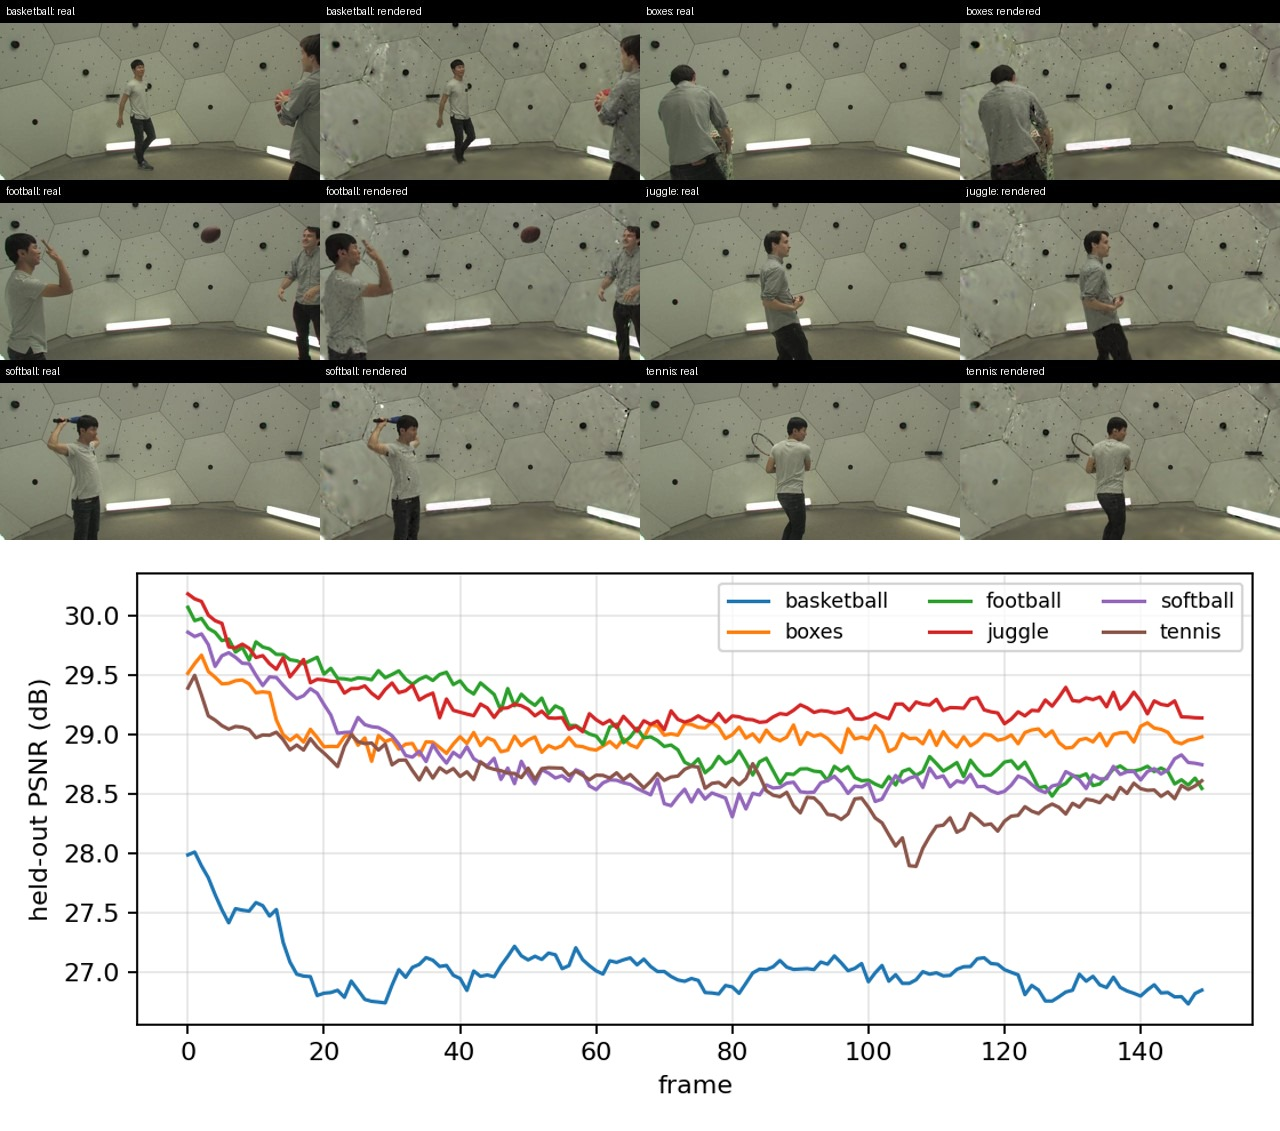
\includegraphics[width=\columnwidth]{heldout_q1.jpg}
\vspace{-1.6em}
\caption{\textbf{Q1, Q2: held-out views.} Top: real vs.\ rendered held-out view at frame 75 for all six sports. Bottom: held-out PSNR for every frame.}
\label{fig:heldout}
\vspace{-1em}
\end{figure}

\noindent\textbf{Q1: held-out quality.} Across all six sports the 4D models score 27.0--29.3\dB PSNR and 0.89--0.91 SSIM on cameras they never saw (\cref{tab:sports}). Real and rendered views are hard to tell apart at a glance (\cref{fig:heldout}); most error sits on the dome walls. Our basketball run is 1.6--2.3\dB below the released models on the other clips; scoring the released basketball model (P1) will show whether that is our training or the clip.

\noindent\textbf{Q2: stability over time.} In every clip PSNR falls by 0.6--1.4\dB over the first frames, while the model moves from the well-fit frame 0 into tracking, and then holds steady: the spread after frame 60 is under 0.2\dB (\cref{fig:heldout}, bottom). So tracking errors do not keep piling up over 150 frames.

\noindent\textbf{Q3: 3D motion.} Because Gaussians persist, every point has a 3D track. Projected into a held-out camera (\cref{fig:tracks}), the tracks follow the real motion: the arc of the thrown football, the loop of the bat and the passes in basketball. The director uses these tracks to find the key moment.

\begin{figure}[t]
\centering
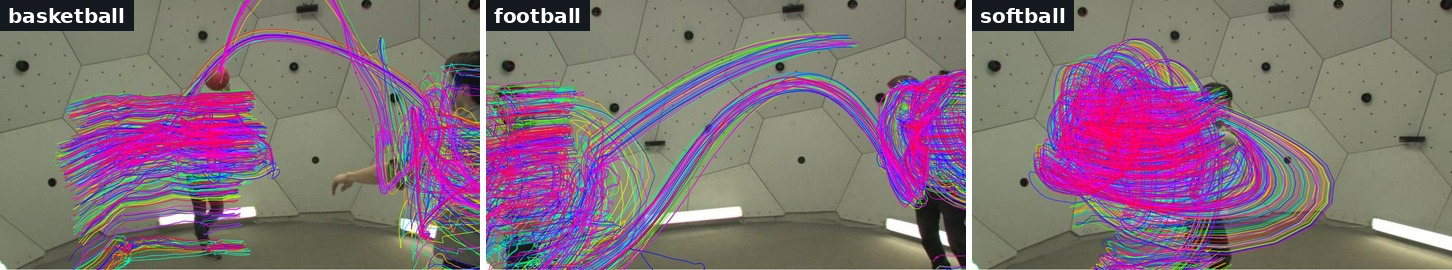
\includegraphics[width=\columnwidth]{tracks.jpg}
\vspace{-1.6em}
\caption{\textbf{Q3: 3D tracks} of 700 moving Gaussians over 150 frames, seen from a held-out camera (basketball, football, softball).}
\label{fig:tracks}
\vspace{-1em}
\end{figure}

\begin{table}[t]
\centering\small
\setlength{\tabcolsep}{3.2pt}
\begin{tabular}{llcccrr}
\toprule
& & \multicolumn{2}{c}{Held-out} & Key & \multicolumn{2}{c}{Jerk$\downarrow$}\\
Clip & Model & PSNR & SSIM & frame & med. & max\\
\midrule
basketball & ours & 27.03 & 0.891 & 59 & 0.020 & 0.237\\
boxes & released & 29.01 & 0.899 & 75$^\ast$ & 0.005 & 0.035\\
football & released & 29.03 & 0.903 & 75 & 0.008 & 0.178\\
juggle & released & 29.28 & 0.908 & 50 & 0.013 & 0.261\\
softball & released & 28.78 & 0.904 & 81 & 0.015 & 0.107\\
tennis & released & 28.60 & 0.904 & 49 & 0.015 & 0.411\\
\midrule
\multicolumn{5}{l}{Naive orbit (blend real camera poses), basketball} & 0.704 & 9.81\\
\bottomrule
\end{tabular}
\vspace{-0.6em}
\caption{\textbf{Results across sports.} Held-out PSNR/SSIM over 150 frames and 4 cameras; the key (freeze) frame the director chose; and camera jerk of the replay (change in global optical-flow motion per frame, px at 320\,px width). $^\ast$No ball in \emph{boxes}: the red-object rule locked onto red box wrapping.}
\label{tab:sports}
\vspace{-1em}
\end{table}

\begin{figure}[t]
\centering
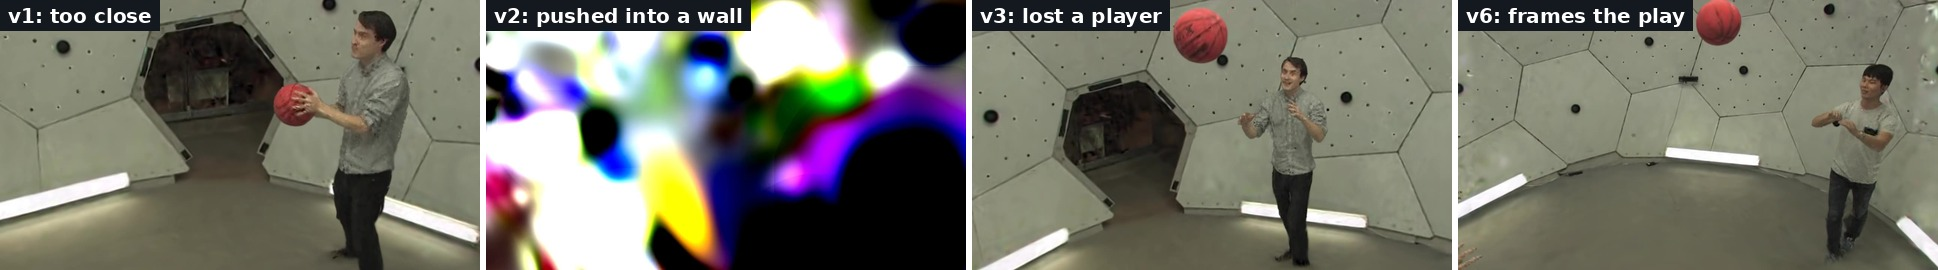
\includegraphics[width=\columnwidth]{director_versions.jpg}
\vspace{-1.6em}
\caption{\textbf{How the director improved} (basketball, same video frame). v1 flew too close; in v2 stray floaters pushed the camera into the wall; v3 dropped the second player; v6 follows the play.}
\label{fig:versions}
\vspace{-1.2em}
\end{figure}

\noindent\textbf{Q4: replays across sports.} We measure smoothness from the video alone, as the per-frame change of the median optical flow (``jerk''). Against a naive orbit that blends real camera poses at a similar speed (0.82 vs.\ 0.76\,px/frame), our basketball replay has 35$\times$ lower median jerk and 41$\times$ lower worst case (\cref{tab:sports}). All six clips stay below 0.42 at worst. The calmest is \emph{boxes}, a slow movement; the hardest are \emph{tennis} and \emph{juggle}, where fast, thin objects make the aim point move quickly. Clearance only pushed the camera out in the two-person clips (75 frames in basketball, 58 in football). The key-moment finder lands within one frame of the truth on synthetic tests (74 vs.\ 75 for a ball apex, 99 vs.\ 100 for a swing). On real clips its red-object rule found a ``ball'' in all six, including \emph{boxes}, where it tracked red wrapping and froze when the stack was tallest. That moment is sensible only by luck, so the rule will be replaced (P4). Two more weaknesses: in \emph{football} and \emph{juggle} the opening shot starts behind the athlete, and thin objects (racket, bat) blur in fast swings.

\noindent\textbf{Planned experiments (to Dec.\ 14).} \textbf{P1} Train all six clips with our own pipeline and score the released basketball model, so every result comes from one setup. \textbf{P2} Sharper fast, thin objects (bat, racket, small balls), \eg finer time steps or extra Gaussians around fast motion. \textbf{P3} 3D accuracy: compare Gaussian tracks with the aligned skeletons. \textbf{P4} A smarter director: use skeletons to pick the key moment and avoid back views, replacing the red-object rule. \textbf{P5} An interactive viewer where the audience picks its own angle. Timeline: P1 by Nov.\ 23, P2--P3 by Dec.\ 5, P4--P5 by Dec.\ 14.

%%%%%%%%%%%%%%%%%%%%%%%%%%%%%%%%%%%%%%%%%%%%%%%%%%%%%%%%%%%%%%%%%%%%%%
\section{Conclusion}
\label{sec:conclusion}

We built an open pipeline that turns synchronized multi-angle video into a cinematic 3D replay, and tested each step. The 4D models match unseen views well (27--29\dB on all six sports), stay stable over time and track the athletes' motion in 3D, and the director turns them into smooth replays without per-clip tuning. \textbf{Limitations:} five replays use released models; fast, thin objects blur; some opening shots start behind the athlete; and a lab dome is smaller and better lit than a stadium. Next we close these gaps and make the replay interactive.

{\small
\bibliographystyle{ieeenat_fullname}
\bibliography{main}
}
\end{document}
